\documentclass{article}
\usepackage[utf8x]{inputenc}
\usepackage{ucs}
\usepackage{amsmath} 
\usepackage{amsfonts}
\usepackage{marvosym}
\usepackage{wasysym}
\usepackage{upgreek}
\usepackage[english,russian]{babel}
\usepackage{graphicx}
\usepackage{float}
\usepackage{textcomp}
\usepackage{hyperref}
\usepackage{geometry}
  \geometry{left=2cm}
  \geometry{right=1.5cm}
  \geometry{top=1cm}
  \geometry{bottom=2cm}
\usepackage{tikz}
\usepackage{ccaption}
\usepackage{multicol}

\hypersetup{
   colorlinks=true,
   citecolor=blue,
   linkcolor=black,
   urlcolor=blue
}

\usepackage{listings}
%\setlength{\columnsep}{1.5cm}
%\setlength{\columnseprule}{0.2pt}

\usepackage[absolute]{textpos}

\usepackage{colortbl,graphicx,tikz}
\definecolor{X}{rgb}{.5,.5,.5}


\begin{document}
\pagenumbering{gobble}
\lstset{
  language=C,                % choose the language of the code
  basicstyle=\linespread{1.1}\ttfamily,
  columns=fixed,
  fontadjust=true,
  basewidth=0.5em,
  keywordstyle=\color{blue}\bfseries,
  commentstyle=\color{gray},
  stringstyle=\ttfamily\color{orange!50!black},
  showstringspaces=false,
  numbersep=5pt,
  numberstyle=\tiny\color{black},
  numberfirstline=true,
  stepnumber=1,                   % the step between two line-numbers.        
  numbersep=10pt,                  % how far the line-numbers are from the code
  backgroundcolor=\color{white},  % choose the background color. You must add \usepackage{color}
  showstringspaces=false,         % underline spaces within strings
  captionpos=b,                   % sets the caption-position to bottom
  breaklines=true,                % sets automatic line breaking
  breakatwhitespace=true,         % sets if automatic breaks should only happen at whitespace
  xleftmargin=.2in,
  extendedchars=\true,
  keepspaces = true,
}
\lstset{literate=%
   *{0}{{{\color{red!20!violet}0}}}1
    {1}{{{\color{red!20!violet}1}}}1
    {2}{{{\color{red!20!violet}2}}}1
    {3}{{{\color{red!20!violet}3}}}1
    {4}{{{\color{red!20!violet}4}}}1
    {5}{{{\color{red!20!violet}5}}}1
    {6}{{{\color{red!20!violet}6}}}1
    {7}{{{\color{red!20!violet}7}}}1
    {8}{{{\color{red!20!violet}8}}}1
    {9}{{{\color{red!20!violet}9}}}1
}
\newpage

\title{Семинар \#11: Динамический массив. Стек и Очередь. Классные задания.\vspace{-5ex}}\date{}\maketitle
\section*{Часть 1: Сегменты памяти}
\begin{multicols}{2}
\begin{center}
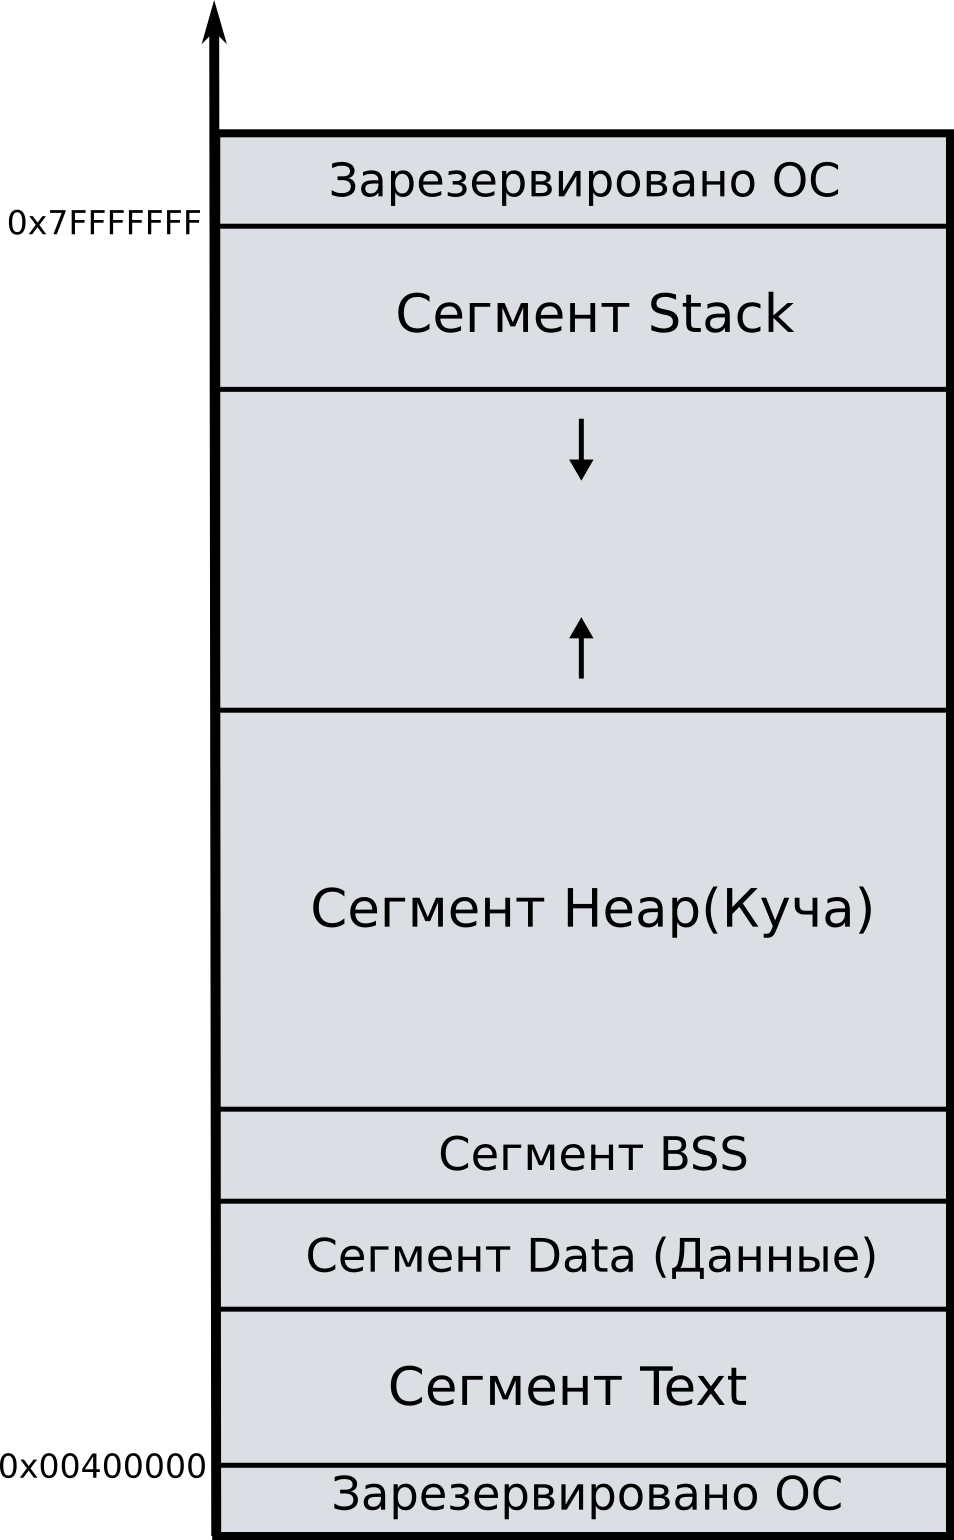
\includegraphics[scale=1.1]{../images/memory_layout.png}
\end{center}
\columnbreak
\begin{enumerate}
\item \textbf{Сегмент памяти Стек (Stack)} \\
\begin{itemize}
\item При обычном объявлении переменных и массивов все они создаются в стеке: 
\begin{lstlisting}
int a; 
int array[10];
\end{lstlisting}


\item Память на локальные переменные функции выделяется при вызове этой функции и освобождается при завершении функции.
\item Маленький размер (несколько мегабайт, зависит от настроек операционной системы).
\item Выделение памяти происходит быстрее чем в куче
\end{itemize}
\item \textbf{Сегмент памяти Куча (Heap)} \\
\begin{itemize}
\item Выделеть память в куче можно с помощью стандартной функции \texttt{malloc}. \\
\begin{lstlisting}
int* p = malloc(10 * sizeof(int));
\end{lstlisting}
\item Освободить память в куче можно с помощью стандартной функции \texttt{free}
\begin{lstlisting}
free(p);
\end{lstlisting}
\item Память можно выделяется/освобождать в любом месте.
\item Размер ограничен свободной оперативной памятью.
\item Выделение памяти происходит медленней чем в стеке
\end{itemize}
\end{enumerate}
\end{multicols}

\begin{enumerate}
\setcounter{enumi}{2}

\item \textbf{Сегмент памяти Data}
\begin{itemize}
\item В этом сегменте хранятся инициализированные глобальные и статические переменные а также строковые литералы
\end{itemize}

\item \textbf{Сегмент памяти BSS}
\begin{itemize}
\item В этом сегменте хранятся неинициализированные глобальные и статические переменные
\item В большинстве систем все эти данные автоматически инициализируются нулями
\end{itemize}

\item \textbf{Сегмент памяти Text}
\begin{itemize}
\item В этом сегменте хранится машинный код программы (Код на языке C, сначала, переводится в код на языке Ассемблера, а потом в машинный код. Как это происходит смотрите ниже.).
\item Адрес функции - адрес первого байта инструкций в этом сегменте.
\end{itemize}
\end{enumerate}


\subsection*{Создание массива в разных сегментах памяти}
Ниже представлен пример программы в которой создаюся 4 массива в разных сегментах памяти.
\begin{lstlisting}
#include <stdio.h>
#include <stdlib.h>

int array_data[5] = {1, 2, 3, 4, 5};
int array_bss[5];

int main() 
{
    int array_stack[5];
    int* array_heap = (int*)malloc(5 * sizeof(int));
}
\end{lstlisting}
\begin{itemize}
\item Напечатайте адрес начала каждого из массивов. Помните, что для печати адресов используется спецификатор \texttt{\%p}.
\end{itemize}



\subsection*{Переполнение стека -- Stackoverflow}
\begin{itemize}
\item Определите размер стека на вашей системе экспериментальным путём. Создайте массив такого большого размера на стеке, чтобы перестала работать. Минимальный размер массива, при котором падает программа будет примерно равен размеру стека.
\item При каждом вызове функции в стеке хранятся локальные переменные функции, аргументы функции а также адрес возврата функции. Даже функция без локальных переменных и аргументов будет хранить на стеке как минимум адрес возврата (8 байт). Определите размер стека на вашей системе экспериментальным путём с помощью рекурсии.
\end{itemize}

\subsection*{Статические переменные}
Помимо глобальных переменных, в сегменте Data хранятся статические переменные. Такие переменные объявляются внутри функций, но создаются в сегменте Data и не удаляются при завершении функции. Вот пример функции со статической переменной.
\begin{lstlisting}
#include <stdio.h>
void counter() {
    static int n = 0;
    n++;
    printf("%i\n", n);
}

int main() {
    counter();
    counter();
    counter();
}
\end{lstlisting}
Обратите внмание, что в этой функции строка \texttt{static int n = 0;} не исполняется при заходе в функцию. Эта строка просто объявляет инициализирует статическую переменную, причём инициализация происходит в самом начале исполнения программы (даже до функции \texttt{main}). 

\begin{itemize}
\item Создайте функцию \texttt{adder}, которая будет принимать на вход число и возвращать сумму всех чисел, которые приходили на вход этой функции за время выполнения программы.
\begin{lstlisting}
printf("%i\n", adder(10));  // Напечатает 10
printf("%i\n", adder(15));  // Напечатает 25
printf("%i\n", adder(70));  // Напечатает 95
\end{lstlisting}
\end{itemize}

\newpage
\section*{Часть 2: Статический массив внутри структуры}
В файле \texttt{0array\_in\_struct.c} содержится минимальный пример массива, который хранится внутри структуры. Максимальная вместимость массива равна \texttt{100}. А размер хранится внутри структуры и может принимать значения от 0 до 100. Функция \texttt{push\_back} принимает на вход адрес на такую структуру и число \texttt{value}, а затем добавляет это число в конец массива.\\

Зачем хранить массив внутри структуры, если можно было бы просто создать его без струтуры? На самом деле у такого подхода много преимуществ:
\begin{enumerate}
\item Он позволяет нам самим описать поведение массива при добавлении и удалении элементов.
\item Мы можем передавать такой массив внутри функций также как и обычные переменные.
\item Такой подход распространяется на более сложные структуры данных
\end{enumerate}

\subsection*{Задачи:} 
Напишите следующие функции для работы с этим массивом:
\begin{itemize}
\item \texttt{array\_print} -- эта функция должна принимать на вход адрес структуры \texttt{Array} и печатать массив на экран.
\item \texttt{array\_is\_empty} -- эта функция должна принимать на вход адрес структуры \texttt{Array} и возвращать \texttt{1}, если массив пуст и \texttt{0} иначе.
\item \texttt{int array\_get(const Array* a, int index)} эта функция должна возвращать число, которое лежит по индексу \texttt{index} в массиве.
\item \texttt{void array\_set(const Array* a, int index, int value)} -- эта функция должна устанавливать элемент массива, лежащий по индексу \texttt{index} значением \texttt{value}.
\item \texttt{void array\_erase(const Array* a, int index)} -- эта функция должна удалять элемент под индексом \texttt{index}. При этом, конечно, все элементы, которые следовали после удаляемого нужно сместить влево на 1 элемент.
\item \texttt{void array\_insert(const Array* a, int index)} -- эта функция должна вставлять элемент в массив в место между элементами с индексами \texttt{index - 1} и \texttt{index}. При этом, конечно, все элементы, которые находились правее этого места, должны сместиться вправо на один элемент.
\item \texttt{void array\_append(Array* a, const Array* b)} -- эта функция должна добавлять всё содердимое массива \texttt{b} в конец массива \texttt{a}.

\item \textbf{Проверка индекса:} Как известно, в языке \texttt{C} у статических массивов нет проверки на выход за пределы массива. Например, следующий код может сработать и не выдасть никакой ошибки.
\begin{lstlisting}
int array[100] = {};
printf("%i\n", array[101]);
\end{lstlisting}
Компилятор просто преобразует строку \texttt{array[101]} в \texttt{*(array + 101)} и обратится к соответствующему участку памяти.
Причина того, что в \texttt{C} нет такой проверки заключается в том, что она бы немного замедлила программу. Язык \texttt{C} ориентирован на максимальное быстродействие, поэтому и не делает такую проверку. 

Однако, за отсутствие такой проверки приходится платить тем что в программе могут появиться сложно выявляемые ошибки. Например, если вы случайно ошибётесь с индексами массива, то можете этого даже не заметить. Программа будет работать с памятью за пределами этого массива и почти всегда выдавать правильные результаты. Но иногда, выходя за пределы массива вы можете изменить другие переменные. Найти такую ошибку в большой программе может быть очень сложно.

Добавьте в нашу реализацию массива проверку на принадлежность индекса правильному диапазону значений в функции \texttt{array\_get} и \texttt{array\_set}. Если индекс не входит в правильный диапазон, программа должна печатать сообщение об ошибке и завершаться. Завершить программу можно с помощью вызова \texttt{exit(1)}, функции \texttt{exit} из библиотеки \texttt{stdlib.h}. 

\item \textbf{Вместимость:} Текущая вместимость нашего массива -- всего 100 элементов. Если размер массива превысит это значение, то тоже должна происходить ошибка. Добавьте проверку на превышение вместимости в функции \texttt{array\_insert} и \texttt{array\_append}. Чтобы не писать везде магическое число \texttt{100}, введите константу, которая будет задавать вместимость.

\end{itemize}

\newpage
\section*{Часть 3: Динамический массив}
У статического массива есть 2 очень больших недостатка:
\begin{itemize}
\item[--] Во-первых, он выделяется на стеке и его размер сильно ограничен.
\item[--] Во-вторых, его вместимость является постоянным числом и не может меняться в процессе выполнения программы. Это всё ведёт к неэффективному использованию памяти, так как мы обязаны задавать размер статического массива таким, чтобы в него всё влезло при любых входных данных.
\end{itemize}

Эти проблемы исправляются в динамическом массиве. Структура для динамического массива выглядит следующим образом:
\begin{lstlisting}
#include <stdio.h>
struct dynarray 
{
    size_t size;
    size_t capacity;
    int* values;
};
typedef struct dynarray Dynarray;
\end{lstlisting}
В этой структуре \texttt{size} означает размер массива (как и прежде). \texttt{capacity} означает текущую вместимость массива, в отличии от статического массива эта величина может меняться. \texttt{values} -- это указатель на элементы массива, которые выделяются в куче. Количество памяти, выделенной в куче, всегда равно \texttt{capacity * sizeof(int)}.\\

\subsection*{Задачи:} 
Напишите следующие функции для работы с динамическим массивом:
\begin{itemize}
\item \texttt{Dynarray dynarray\_create(size\_t initial\_capacity)} -- эта функция должна создавать динамический массив с размером равным нулю и вместимостью равной \texttt{initial\_capacity}. Память должна выделяться в куче с помощью \texttt{malloc}.

\item \texttt{void dynarray\_destroy(Dynarray* d)} -- эта функция должна освобождать выделенную память (\texttt{free}).

\item Перепишите все функции из прошлой части: \texttt{dynarray\_push\_back}, \texttt{dynarray\_print} и другие.

\item \textbf{Расширение массива:} Измените код так, чтобы происходило перевыделение памяти тогда, когда размер массива начинает превышать вместимость в функциях \texttt{dynarray\_push\_back} и \texttt{dynarray\_insert}. Вместимость динамического массива должна увеличиваться в 2 раза.  Это можно сделать двумя способами:
\begin{itemize}
\item Выделить новый участок памяти в 2 раза больше прежнего, используя \texttt{malloc}. Переписать все элементы в новую память. Освободить старую память с помощью \texttt{free}.
\item Использовать функцию \texttt{realloc}, которая будет делать то же самое, но более эффективно.
\end{itemize}

\item \textbf{Проверка на корректность:} Функции \texttt{malloc} и \texttt{realloc} не всегда могут выделить необходимую память. Например, если вы запросите больше чем вся оперативная память, то они ничего не смогут сделать. В этом случае эти функции возвращают нулевой указатель (т.е. указатель, равный \texttt{NULL}). В случае возникновения такой ошибки \texttt{realloc} не освобождает старую память. Добавьте в программу проверки на возникновения таких ошибок. Если память выделить нельзя, то программа должна печатать сообщение о нехватке памяти и завершаться.

\item \textbf{Размер и вместимость:}
Напишите программу, которая будет создавать стек вместимости \texttt{1} и добавлять в него последовательно \texttt{200} элементов. При каждом добавлении элемента печатайте размер и вместимость.\\

\item \textbf{Другие типы элементов:} Предположим, что вы однажды захотите использовать динамический массив не для целочисленных чисел типа \texttt{int}, а для какого-нибудь другого типа (например \texttt{char}). Введите синоним для типа элементов динамического массива:
\begin{verbatim}
typedef int Data;
\end{verbatim}
Измените тип элемента динамического массива во всех функциях с \texttt{int} на \texttt{Data}. Теперь вы в любой момент сможете изменить тип элементов стека, изменив лишь одну строчку.
\end{itemize}


\newpage
\section*{Часть 4: Заголовочные файлы}


\newpage
\section*{Часть 5: Абстрактные типы данных: Стек и Очередь, Дек и Очередь с приоритетом}
\textbf{Абстракстный тип данных (АТД)} - это математическая модель для типов данных, которая задаёт поведение этих типов, но не их внутреннею реализацию.\\

\textbf{Стек (Stack, не путайте с сегментом памяти под таким же названием!)} - это АТД, который представляет собой коллекцию элементов, менять которые можно только с помощью двух операций:
\begin{itemize}
\item \texttt{push} - добавить элемент в стек.
\item \texttt{pop} - извлечь из стека последний добавленный элемент.
\end{itemize}
Таким образом, поведение стека задаётся этими двумя операциями. Так как стек - это абстрактный тип данных, то его внутренняя реализация на языке программирования может быть самой разной. Стек можно сделать на основе статического массива, на основе динамического массива или на основе связного списка. Внутренняя реализация не важна, важно только наличие операций \texttt{push} и \texttt{pop}. \\
Не нужно путать абстракстный тип данных стек с сегментом памяти стек.\\

\textbf{Очередь (Queue)} - это АТД, который представляет собой коллекцию элементов, менять которые можно только с помощью двух операций:
\begin{itemize}
\item \texttt{enqueue} - добавить элемент в очередь.
\item \texttt{dequeue} - извлечь из очереди первый добавленный элемент из оставшихся.
\end{itemize}

\begin{center}
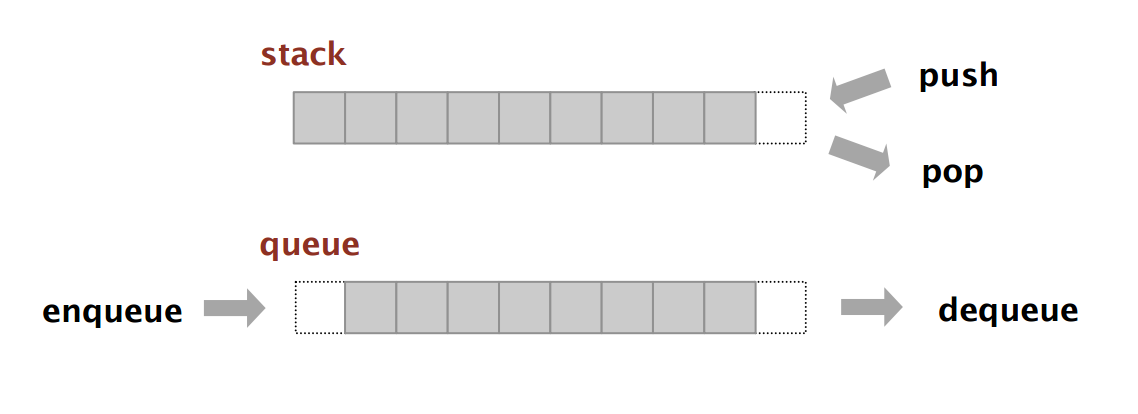
\includegraphics[scale=0.31]{../images/stack_queue.png}
\end{center}

\textbf{Дек (Deque = Double-ended queue)} - это АТД, который представляет собой коллекцию элементов, менять которые можно только с помощью четырёх операций:
\begin{itemize}
\item \texttt{push\_back} - добавить элемент в конец.
\item \texttt{push\_front} - добавить элемент в начало.
\item \texttt{pop\_back} - извлечь элемент с конца.
\item \texttt{pop\_front} - извлечь элемент с начала.\\
\end{itemize}

\textbf{Очередь с приоритетом (Priority Queue)} - это АТД, который представляет собой коллекцию элементов, менять которые можно только с помощью двух операций:
\begin{itemize}
\item \texttt{insert} - добавить элемент.
\item \texttt{extract\_best} - извлечь из очереди элемент с наибольшим приоритетом. 
\end{itemize}
То, что будет являться приоритетом может различаться. Это может быть как сам элемент, часть элемента (например, одно из полей структуры) или другие данные, подаваемые на вход операции \texttt{insert} вместе с элементом. В простейшем случае, приоритетом является сам элемент (тогда очередь с приоритетом просто возвращает максимальный элемент) или сам элемент со знаком минус (тогда очередь с приоритетом возвращает минимальный элемент).


\newpage
\section*{Часть 6: Реализация стека на основе динамического массива}

\begin{center}
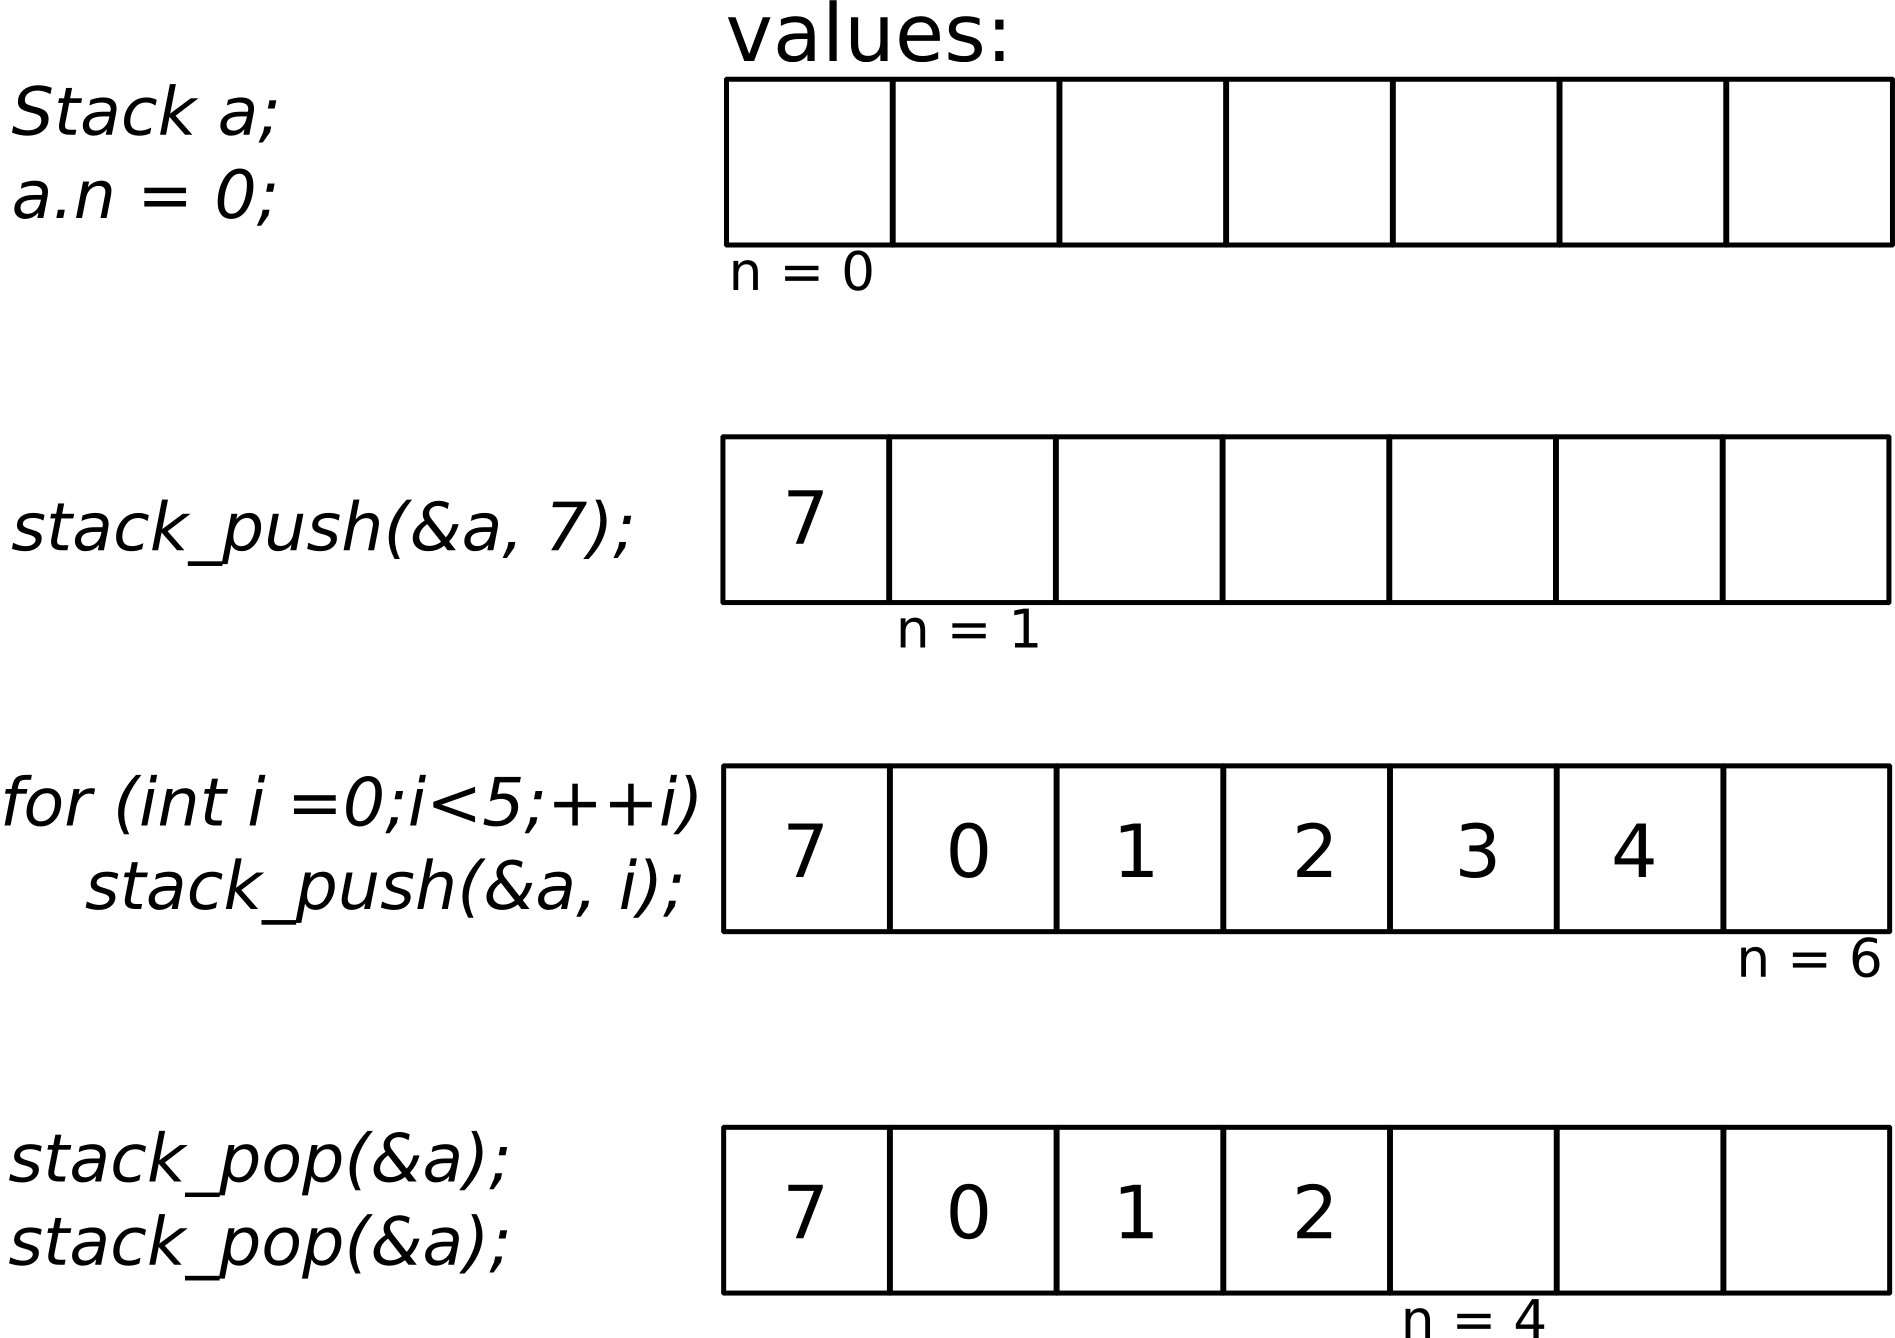
\includegraphics[width=0.6\linewidth]{../images/stack.png}
\end{center}

\subsection*{Задачи:}
\begin{itemize}
\item Напишите следующие функции:
\begin{enumerate}
\item \texttt{void stack\_push(Stack* s, Data x)} -- добавляет элемент в стек.
\item \texttt{Data stack\_get(const Stack* s)} -- возвращает элемент, находящийся в вершине стека, но не изменяет стек.
\item \texttt{void stack\_pop(Stack* s)} -- удаляет элемент, находящийся в вершине стека. 
\item \texttt{int stack\_is\_empty(const Stack* s)} -- возвращает 1 если стек пуст и 0 иначе.
\item \texttt{void stack\_print(const Stack* s)} -- распечатывает все элементы стека.
\end{enumerate}



\item \textbf{Скобочки}: Написать программу которая будет считывать последовательность скобочек и
печатать \texttt{Yes} или \texttt{No} в зависимости от того является ли эта последовательность допустимой. Для считывания строки: \texttt{scanf(``\%s'', str);}
\begin{multicols}{2}
\begin{center}
\begin{tabular}{ c | c }
 вход & выход \\ \hline
 \texttt{()} & Yes \\
 \texttt{\{[()]\}} & Yes  \\ 
 \texttt{)))))}  &  No \\ 
 \texttt{([)]}  &  No \\ 
 \texttt{[\{\}()]}  &  Yes \\ 
\end{tabular}
\end{center}

\begin{center}
\begin{tabular}{ c | c }
 вход & выход \\ \hline
 \texttt{)(}  &  No \\
 \texttt{((((((()))))))} & Yes \\
 \texttt{\{\{\{\{} & No  \\ 
 \texttt{\{[([]()[\{\}])][()]\}}  &  Yes \\ 
 \texttt{]}  &  No \\ 
\end{tabular}
\end{center}
\end{multicols}


\item \textbf{Следующий больший}: На вход поступает последовательность чисел. Нужно найти, для каждого элемента, индекс первого элемента, который следует после данного и является больше данного. Если такого элемента нет, то нужно напечатать \texttt{-1}.
\begin{center}
\begin{tabular}{ l | l }
 вход & выход \\ \hline
 \texttt{10} &  \texttt{1 4 3 4 5 -1 7 -1 -1 -1}\\
 \texttt{1 5 2 4 6 9 1 8 7 3} & \\ \hline
 
 \texttt{5} &  \texttt{1 2 3 4 -1}\\
 \texttt{1 2 3 4 5} & \\ \hline
 
  \texttt{2} &  \texttt{-1 -1}\\
 \texttt{2 1} & \\
\end{tabular}
\end{center}

\end{itemize}
\end{document}